\documentclass[12pt]{article}

\usepackage{pgfplots}
\pgfplotsset{compat=1.18} % Or adjust depending on your TeX distribution
\usepackage[utf8]{inputenc}	% Para caracteres en español
\usepackage{amsmath,amsthm,amsfonts,amssymb,amscd}
\usepackage{multirow,booktabs}
\usepackage[table]{xcolor}
\usepackage{fullpage}
\usepackage{lastpage}
\usepackage{newtxtext}
\usepackage{newtxmath}
\usepackage{enumitem}
\usepackage{fancyhdr}
\usepackage{mathrsfs}
\usepackage{wrapfig}
\usepackage{setspace}
\usepackage{calc}
\usepackage{multicol}
\usepackage{cancel}
\usepackage[retainorgcmds]{IEEEtrantools}
\usepackage[margin=3cm]{geometry}
\usepackage{amsmath}
\newlength{\tabcont}
\setlength{\parindent}{0.0in}
\setlength{\parskip}{0.05in}
\usepackage{empheq}
\usepackage{framed}
\usepackage[most]{tcolorbox}
\usepackage{xcolor}
\colorlet{shadecolor}{orange!15}
\parindent 0in
\parskip 12pt
\geometry{margin=1in, headsep=0.25in}
\theoremstyle{definition}
\newtheorem{defn}{Definition}
\newtheorem{reg}{Rule}
\newtheorem{exer}{Exercise}
\newtheorem{note}{Note}
\newtheorem{theorem}{Theorem}
\setcounter{section}{0}
\usepackage{chngcntr}
\usepackage{hyperref}
\counterwithin*{equation}{section}
\counterwithin*{equation}{subsection}


\begin{document}

\section{Info}

\begin{itemize}
    \item karinachattah@unc.edu.ar
\end{itemize}

\textbf{Temas:}

\begin{itemize}
    \item Cinemática y dinámica (mecánica)
    \item Campos eléctricos y magnéticos
    \item Circuitos 
    \item Termodinámica
\end{itemize}

\section{Measurements and magnitudes}

Measurements seek to compare a prediction with an observation, so as to test a
hypothesis. A magnitude is a number accompanied by a unit. Some magnitudes are: 

\begin{itemize}
    \item Length, measured in meters $(m)$
    \item Time, measured in seconds ($s$)
    \item  Mass, measusred in kilograms (kg)
    \item Current, measured in ampers ($A$)
    \item Temperature, measured in kelvins ($k$)
    \item Matter, measured in moles (mol)
\end{itemize}

We consider $10^3$ (e.g. kilometer) and $10^{-3}$ (e.g. milimiters) to be within
human scale.  We call mass, seconds and kilograms the \textit{mechanical units}.
We define the \textit{force unit}, or Newton, as

\begin{equation*}
    [F] = N = \text{kg} \frac{m}{s^2}
\end{equation*}

and the Pascal unit as 

\begin{equation*}
    [P] = \text{Pa} = \frac{N}{m^2}
\end{equation*}

We use scientific notation and terms which express quantities as powers of ten.
For instance, $10^{12}$ is the tera, $10^{3}$ the giga, etc.

The magnitudes hereby described are suited for algebraic manipulation. For
instance, $m \times m = m^2$, and $s \times \frac{m}{s} = m$.

\section{Vectors}

Vectors are used to express position, displacement, velocity, force,
acceleration, fields, etc. A vector $\overrightarrow{A}$ (or sometimes
$\overrightarrow{a}$) in the general sense has a direction (line), an
orientation, and a length (or magnitude). A vector also has an application
point, which denotes the point of origin of the vector. When saying $\overrightarrow{a}
= \overrightarrow{b}$, we mean that $\overrightarrow{a}$ and
$\overrightarrow{b}$ coincide in direction, magnitude and orientation,
irrespective of their application point. 

The scalar product is defined as the usual mapping in the space $\mathbb{R}^n
\times \mathbb{R} \mapsto \mathbb{R}^n$. Intuitively, the scalar product $\lambda
\overrightarrow{a}$
"streches" or "shrinks" a vector, depending on wheter $|\lambda| < 1$ or not,
and the positivty or negativity of $\lambda$ determines whether the vector
inverts its direction or not. In general, $\left| \lambda \overrightarrow{a}
\right| = \left| \lambda \right| \left| \overrightarrow{a} \right| $.

The sum of vectors, $\overrightarrow{a} + \overrightarrow{b}$, is a mapping
$\mathbb{R}^n \times \mathbb{R}^n \mapsto \mathbb{R}^n$. As usual, and in a
graphical sense, the sum corresponds to the application of the parallelogram
rule. 

\begin{shaded}
    \textbf{Parallelogram rule}. Make $\overrightarrow{a}$ and
    $\overrightarrow{b}$ coincide in their point of application. From the tip of 
    $\overrightarrow{a}$, draw a copy of $\overrightarrow{b}$, and from the tip
    of $\overrightarrow{b}$ a copy of $\overrightarrow{a}$. The corner of the
    thus generated parallelogram is the tip of $\overrightarrow{a} +
    \overrightarrow{b}$.

    Alternatively, from the tip of $\overrightarrow{a}$ write
    $\overrightarrow{b}$. Then $\overrightarrow{a} + \overrightarrow{b}$ is the
    vector which goes from the point of application of $\overrightarrow{a}$ to
    the tip of $\overrightarrow{b}$.
\end{shaded}

The sum of vectors is commutative, associative, and distributive with respect to
scalar product.

If $\overrightarrow{A}$ is a vector, we use $A_x$ and $A_y$ to denote the
projection of the vector over the axis $x$ or $y$, respectively. Using $A_x$ and
$A_y$ one forms a rectangular triangle with sides $A_x$, $A_y$ and a hypotenuse 
of length $\left| \overrightarrow{A} \right| $. 

Let $\theta$ be the angle formed
by $\overrightarrow{A}$ with the $x$-axis. Then, using trigonometry,

\begin{equation*}
    \cos \theta = \frac{A_x}{\left| \overrightarrow{A} \right| }, \qquad \sin
    \theta = \frac{A_y}{\left| \overrightarrow{A} \right| }
\end{equation*}

from which one can find $A_x, A_y$ assuming one knows $\theta$. From this
follows that $\left| \overrightarrow{A} \right| $ and $\theta$ fully determine
all the information about the vector, insofar as the allow us to determine $A_x,
A_y$. Conversely, knowing $A_x$ and $A_y$ is also sufficient to determine
$\overrightarrow{A}$, insofar as 

\begin{equation*}
    \left| \overrightarrow{A} \right|  = \sqrt{A_x^2 + A_y^2} , \qquad \frac{A_y}{A_x} =
    \frac{\left| \overrightarrow{A} \right| \sin \theta}{\left|
    \overrightarrow{A} \right|  \cos \theta} = \tan \theta \Rightarrow \theta =
    \arctan \left( \frac{A_y}{A_x} \right) 
\end{equation*}

As convention, we use $\hat{i}$ to denote the versor (vector of length 1) with
direction parallel to the $x$-axis, and $\hat{j}$ the versor with direction
parallel to the $y$-axis.

Notice that, for any vector $\overrightarrow{A}$, $A_x$ is $\hat{i}$ times
$A_x$, and $A_y$ is $\hat{j}$ times $A_y$, which means 

\begin{equation*}
    \overrightarrow{A} = A_x \hat{i} + A_y \hat{j}
\end{equation*}

When writing $\overrightarrow{A}$ in this way, we say we write it in term of its
components $x, y$. In terms of linear algebra, it's not hard to see that we are
simply expressing that $\hat{i}, \hat{j}$  form a basis of $\mathbb{R}^2$. Thus,
it is equivalent to write 

\begin{equation*}
    A_x = \left| \overrightarrow{A} \right|  \cos \theta, \qquad A_y = \left|
    \overrightarrow{A} \right| \sin \theta
\end{equation*}

and 

\begin{equation*}
    \overrightarrow{A} = \left| \overrightarrow{A} \right| \left( \cos \theta
    ~ \hat{i} + \sin \theta ~ \hat{j}\right) 
\end{equation*}

From this follows as well that 

\begin{align*}
    \overrightarrow{A} + \overrightarrow{B} 
    &= \left( A_x \hat{i} + A_y \hat{j} \right) + (B_x \hat{i} + B_y \hat{j}) \\ 
    &= \hat{i}\left( A_x + B_x \right)  + \hat{j}\left( A_y + B_y \right) 
\end{align*}

which means the sum of vectors has as components the sum of the components.

The scalar product of two vectors, $\overrightarrow{A} \cdot
\overrightarrow{B}$, is a scalar defined as 

\begin{equation*}
    \overrightarrow{A} \cdot \overrightarrow{B} = \left| \overrightarrow{A} \right| \left| \overrightarrow{B} \right| \cos \theta
\end{equation*}

where $\theta$ is the angle formed by the two vectors. The scalar product is
positive if $\cos \theta$ is positive, which occurs for $0 < \theta \leq 90$. It
is negative if $\cos \theta $ is negative, i.e. if $90 < \theta \leq 180$.
Clearly, $\overrightarrow{A} \cdot \overrightarrow{B} = 0 \iff \theta = 90$.

In general, from the definition follows that

\begin{equation*}
    \overrightarrow{A} \cdot \overrightarrow{B} = A_x B_x + A_y B_y
\end{equation*}

The vectorial product $\overrightarrow{A} \times \overrightarrow{B}$ is a vector
perpendicular to the plane formed by $\overrightarrow{A}$ and
$\overrightarrow{B}$. Its module is $\left| \overrightarrow{A} \right| \left|
\overrightarrow{B} \right| \sin \theta $, and its direction is given by what's
called the right-hand rule.

\pagebreak 

\subsection{Excercises}

\begin{shaded}
    \textbf{(2)} Sean los vectores $\overrightarrow{A} = 2\hat{i} + 3\hat{j}$
    $\overrightarrow{B} = 4\hat{i} -2 \hat{j}$ y $\overrightarrow{C} = -\hat{i}
    + \hat{j}$.
    Determinar la magnitud y el ángulo (representación polar) de los vectores
    resultantes $\overrightarrow{D} = \overrightarrow{A} + \overrightarrow{B} +
    \overrightarrow{C}$ y $\overrightarrow{E} = \overrightarrow{A} +
    \overrightarrow{B} - \overrightarrow{C}$. Resolver analítica y
    gráficamente.
\end{shaded}

(Analytical solution.) We'll use $A_x, A_y$ to denote the components of the
vector $\overrightarrow{A}$, and same for all other vectors. We know the
components of $\overrightarrow{D}$ are 

\begin{equation*}
    D_x = A_x + B_x + C_x = 2 + 4 - 1 = 5, \qquad D_y = 3 - 2 + 1 = 2
\end{equation*}

from which readily follows that $\left| D \right| = \sqrt{5^2 + 2^2} = \sqrt{29}
\approx 5.385$. Similarly, 

\begin{equation*}
    E_x = 2 + 4 + 1 = 7, \qquad E_y = 3 - 2 -1 = 0
\end{equation*}

from which follows that $\left| E \right| = \sqrt{7^2} = 7 $.

Now, we must recall that 

\begin{equation*}
    \theta_{\overrightarrow{Z}} = \arctan \left( \frac{Z_y}{Z_x} \right) 
\end{equation*}

for any $\overrightarrow{Z}$.


We need not memorize this: it is trigonometrically clear that 
$Z_x = \cos \theta_{\overrightarrow{Z}} \left| \overrightarrow{Z} \right| $ and 
$Z_y = \sin \theta_{\overrightarrow{Z}} \left| \overrightarrow{Z} \right| $, and
therefore 

\begin{equation*}
    \frac{Z_y}{Z_x} = \tan \theta
\end{equation*}

And $\arctan$ is the inverse of $\tan$. Anyhow, for $\overrightarrow{E}$ and
$\overrightarrow{D}$ we have 

\begin{equation*}
    \theta_{\overrightarrow{E}} = \arctan\left( \frac{E_y}{E_x} \right) =
    \arctan\left( 0 \right) = 0
\end{equation*}

\begin{equation*}
    \theta_{\overrightarrow{D}} = \arctan\left( \frac{D_y}{D_x} \right) =
    \arctan \left( \frac{2}{5} \right) \approx 0.38
\end{equation*}

\pagebreak 

\begin{shaded}
    \textbf{(3)} Can two vectors of different magnitud be combined and yield zero? What about three?
\end{shaded}

The zero vector is the only vector with magnitude zero. Let $\overrightarrow{A},
\overrightarrow{B}$ arbitrary vectors. Then 

\begin{equation*}
    \left| \overrightarrow{A} + \overrightarrow{B} \right| = \sqrt{(A_x + B_x)^2
    + (A_y + B_y)^2} 
\end{equation*}

which is zero if and only if 

\begin{equation*}
    ( A_x + B_x )^2 + ( A_y + B_y )^2 = 0
\end{equation*}

This only holds if $A_x + B_x = A_y + B_y = 0$. But 

\begin{equation*}
    A_x + B_x = 0 \Rightarrow A_x = -B_x, \qquad A_y + B_y = 0 \Rightarrow A_y =
    -B_y
\end{equation*}

But then 

\begin{equation*}
    \left| A \right| = \sqrt{A_x^2 + A_y^2} = \sqrt{(-B_x)^2 + (-B_y)^2} =
    \sqrt{B_x^2 + B_y^2}  = \left| B \right| 
\end{equation*} 

$\therefore ~ \left| \overrightarrow{A} + \overrightarrow{B} \right| = 0 \iff
\left| \overrightarrow{A} \right| = \left| \overrightarrow{B} \right| $.

It is simple to see that three vectors of different magnitude can add to zero.

\pagebreak 

\begin{shaded}
    Assume $A + B + C = 2\hat{i} + \hat{j}$ and $A = 6\hat{i}-3\hat{j}, B =
    2\hat{i} + 5\hat{j}$. Find the components of $C$. Solve analytically and
    graphically.
\end{shaded}

We know 

\begin{equation*}
    6 + 2 + C_x = 2, \qquad -3 + 5 + C_y = 1
\end{equation*}

from which follows that $C_x = -6, C_y = -1$.

\pagebreak 

\begin{shaded}
    \textbf{(5)} $A$ and $B$ have a magnitud of $3m, 4m$ respectively. The angle between them
    is $\theta = 30$ degrees. Find their scalar product.
\end{shaded}

Their scalar product is 

\begin{equation*}
    ( \left| B \right|  \cos \theta ) \left| A \right| 
\end{equation*}

Recall that 

\begin{equation*}
    \text{Angle in degrees} = \text{Angle in radians} \cdot \frac{180}{\pi}
\end{equation*}

Thus, thirty degrees equates to $30 \frac{\pi}{180} \approx 0.523$ radians. Then
the scalar product is 

\begin{equation*}
    4 \cos (0.523) \times 3 \approx 10.395
\end{equation*}




\pagebreak 

\begin{shaded}
    \textbf{(6)} Find the angle between $A = 4 \hat{i} + 3 \hat{j}$ and 
    $B = 6\hat{i} - 3 \hat{j}$.
\end{shaded}

Recall that 

\begin{equation*}
    A \cdot B = \left| A \right| \left| B \right| \cos \theta
\end{equation*}

where $\theta$ is the angle between the vectors. This readily entails that 

\begin{equation*}
    \frac{A \cdot B}{\left| A \right|\left| B \right|  } = \cos \theta
\end{equation*}

or equivalently that 

\begin{equation*}
    \theta = \arccos \left( \frac{A \cdot B}{\left| A \right|\left| B \right|  } \right)  
\end{equation*}

Now, $A \cdot B = 4 \times 6 + 3 \times -3 = 24 - 9 = 15$ and $\left| A \right|
\left| B \right| = 5 \cdot 6.708 = 33.541 $.

Therefore, 

\begin{equation*}
    \theta = \arccos \left( \frac{15}{33.541} \right) = \arccos \left( 0.447
    \right) = 1.107
\end{equation*}

\pagebreak 

\begin{shaded}
    \textbf{(7)} Let $\overrightarrow{v} = \left( \frac{1}{3}, \frac{2}{3} \right) $ be the vector of
    components. Find the components of the vector of module 5 whose direction 
    and orientation (sentido) are those of the given vector.
\end{shaded}

Assume $\overrightarrow{x} = (x_1, x_2)$ is of magnitude $5$. Any vector whose
direction and orientation are the same than those of $\vec{v}$ is "a stretching"
of $\vec{v}$. In other words, for $\vec{x}$ to satisfy the requirements, we must
have 

\begin{equation}
    \vec{x} = \lambda \vec{y}
\end{equation}

for some $\lambda \in \mathbb{R}$. (Furthermore, $\lambda > 0$ since otherwise
orientation is not preserved.) 

Now, from equation $(1)$ follows that

\begin{equation}
    \|\vec{x}\| =  \lambda \|\vec{y}\|
\end{equation}

since the magnitude of a scaled vector is the scaled magnitude of the vector.
Equation $(2)$ simplifies to 

\begin{equation}
    \|\vec{x}\|  = \lambda \sqrt{1 / 9 + 4 / 9} = \frac{\lambda
    \sqrt{5} }{3}
\end{equation}

From this readily follows that $\frac{3}{\sqrt{5} }\|\vec{x}\| = \lambda$. But
it is a hypothesis that $\|\vec{x}\| = 5$. Therefore, 

\begin{equation}
    \lambda = \frac{3}{\sqrt{5} } \cdot 5 = \frac{15}{\sqrt{5} }
\end{equation}

In other words, 

\begin{equation}
    \vec{x} = \frac{15}{\sqrt{5} } \vec{v} 
\end{equation}

which is ugly but can be simplified.


\pagebreak 

\begin{shaded}
    \textbf{(8)} Write the expression of the vector product $\vec{c} = \vec{u}
    \times \vec{v}$ in the following cases: 

    \begin{enumerate}
        \item $\vec{u}, \vec{v}$ are coplanar. Provide a graphical
            interpretation. 
        \item $\vec{u} = 2\hat{i} - 3 \hat{j} + \hat{k}$ and $\vec{v} =
            -3\hat{i} + \hat{j} + 2 \hat{k}$. Find the module of the resulting
            vector $\vec{c}$ in two different ways.
    \end{enumerate}
\end{shaded}

$(1)$ Two vectors are coplanar if there is a plane which contains them both.
Since the vector product $\vec{u} \times \vec{v}$ is a vector orthogonal 
to both $\vec{u}$ and $\vec{v}$


\pagebreak 

\begin{shaded}
    \textbf{(12)} Un avión vuela 200 km hacia el NE en una dirección que forma
    un ángulo de 30 hacia el este de la dirección norte. En ese punto cambia su
    dirección de vuelo hacia el NO. En esta dirección vuela 60 km formando un
    ángulo de 45 con la direccióon norte.

    (a) Calcular la máxima distancia hacia el este del punto de partida a la que
    llegó el avión. 

(b) Calcular la máxima distancia hacia el norte del punto de partida a la que
llegó el avión. 

(c) Calcular la distancia a la que se encuentra el avión del punto de partida al
cabo de su recorrido. 

(d) Determinar vectorialmente el camino que debería hacer para volver al punto
de partida. Resolver gráfica y analíticamente.
\end{shaded}

Sea $\vec{A}$ el vector que describe el primer recorrido, $\vec{B}$ el
vector que describe el segundo recorrido. Al final del problema, el avión se
encuentra en la posición indicada por $\vec{A} + \vec{B}$. 

Como $\vec{A}$ describe un movimiento con un ángulo de $\theta = 60$ grados
($90 - 30$) respecto al eje $y$ (norte), y una magnitud de 200km, podemos
determinarlo recordando que

\begin{equation*}
     A_x = \left| \vec{A} \right| \cos \theta, \qquad A_y = \left| \vec{A}
     \right| \sin \theta
\end{equation*}

En radianes, $\theta = \frac{\pi}{180} \times 60 = 1.047$

\begin{equation*}
    A_x = 200 \times \cos \left( 1.047 \right) = 100.034, \qquad A_y = 22 \times
    \sin(1.047) = 173.185
\end{equation*}

En conclusión, $\vec{A} = 100.034 \hat{i} + 173.185 \hat{j}$. Mismo razonamiento
nos da que el ángulo del segundo vector es de $130$ grados, lo cual en radianes
nos da $\alpha = \pi / 180 \times 130 = 2.268$. Por ende, 

\begin{equation*}
    B_x = 60 \cos(2.268) = -38.524, \qquad B_y = 60  \sin(2.268) = 45.998
\end{equation*}

Es decir que $\vec{B} = -38.524 \hat{i} + 45.998 \hat{j}$. De esto se sigue 
que $\vec{C} = \vec{A} + \vec{B} = (61.51, 219.183)$. 

$(a)$ Claramente, es la coordenada $x$ del vector $\vec{A}$, $100.034$.

$(b)$ Claramente, es la coordenada $y$ del vector $\vec{C}$: $218.183$. 

$(c)$ Claramente, es la magnitud de $\vec{C}$, es decir $\|\vec{C}\| =
\sqrt{61.51^2 + 219.183^2} = 227.65$.

$(d)$ El camino para volver es dado por $\vec{C} \times (-1)$.

















\pagebreak

\section{Cynematics}


\subsection{Unidimensional movement}

The study of movement requires two variables: position ($x$, in units of length)
and time ($t$, in seconds). We begin our study with unidimensional movement,
i.e. movement which occurs along a single axis. 

Experimentally, a way to study unidimensional movement could consist in taking a
sequence of photographs (from the same position and angle) of the moving object
at times $t_1, \ldots, t_n$. Some coordinate system must be imposed upon the
space along which the object moves, e.g. setting an axis with origin at the
initial position of the object, the same direction as the movement of the
object, and some appropriate units. The photographs would then provide a
sequence of positions $x_1, \ldots, x_n$.

Clearly, $\left\{ t_n \right\}, \left\{ x_n \right\}  $ could be understood as
defining a discrete function $\varphi(n)$, which on its turn might be
interpolated to obtain a continuous approximation $\phi(t)$. To the limit, the
continuous approximation converges to what we call a movement function. 

\begin{shaded}
    \textbf{Movement function}. A movement function $x(t)$ is a continuous,
    smooth function.

    \textbf{Examples.} $x(t) = c$ (reposo), $x(t) = at + b$ (MRU), $x(t) = at^2
    + bt  + c$ (MRUV).
\end{shaded}

\subsection{Coincidence, displacement, temporal intervals}

If $A, B$ are objects with movement functions $x_A(t), x_B(t)$, we say $A, B$
coincide (se encuentran) when $x_A(t) = x_B(t)$.

We define displacement (desplazamiento) (relative to positions $x_1, x_2$) as
$\Delta x = x_2 - x_1$. Notice that $\Delta x$ is not the same as distance: if
one travels from $A$ to $B$ and then to $B$ from $A$, the distance traveled is
to times the distance from $A$ to $B$, but $\Delta x = 0$.

We also define a temporal interval, relative to two times $t_1, t_2$, as $\Delta
t = t_2 - t_1$, where $t_2 > t_1$. 

\subsection{Velocity}

We define \textit{median velocity} (velocidad media) as 

\begin{equation}
    \overline{v} = \frac{\Delta x}{\Delta t} = \frac{x_2 - x_1}{t_2 - t_1}
\end{equation}

where $x_2 = x(t_2), x_1 = x(t_1)$. Clearly, $\overline{v}$ is the slope of the
line which intersects $x(t)$ at points $t_1, t_2$. The sign of $\overline{v}$
then determines the direction (sentido) of movement. The unit of $\overline{v}$
is then $L / T$ (length over time), for instance kilometers per hour. Median
velocity indicates the rate of change of distance in time.

Clearly, an object in reposo has a median velocity of zero. An object with
movement function $x(t) = at + b$ (MRU) has median velocity $a$. The case of
interest is an object with a quadratic movement function (MRUV).

If $x(t) = at^2 + b t + c$, let $m$ the midpoint of the quadratic expression and 
take $t_1 = m - c, t_2 = m + c$ with $c > 0$. Clearly, the median velocity from 
$t_1$ to $m$ is negative, that from $m$ to $t_1$ is positive, and that from 
$t_1$ to $t_2$ is zero. This is sufficient to suggest that median velocity does
not clearly express the nature of the movement. 

For that reason, the length $\Delta$ of the interval $[t_1, t_2]$ might be
reduced in the limit to zero, so that we get an accurate notion of the
instantaneous (or close to instantaneous) change of direction. Needless to say, 
the limit converges to the slope of the line  tangent to $(t_1, x(t_1))$, i.e.
the derivative of $x(t)$ at $t_1$. Thus, we obtain the definition of
instantaneous velocity, usually called simply velocity: 

\begin{equation}
    v(t) = \lim_{\Delta t \to 0} \frac{\Delta x}{\Delta t} = \frac{dx}{dt} =
    v'(t)
\end{equation}

Again, $\left[ v(t) \right] = \frac{L}{T}$. Quite clearly, $v(t) = \overline{v}$
for constant and linear functions, but for the quadratic function $x(t)$ we
have 

\begin{equation*}
    x(t) = at^2 + b t + c, \qquad v(t) = 2at + b
\end{equation*}





\pagebreak
\section{De adelante hacia atrás}

Recordemos que si $x(t)$ es función de movimiento, $v(t) = \frac{dx}{dt}$ es la
velocidad, y $a(t) = \frac{d^2 x}{dt^2}$ es la aceleración. Naturalmente, esto
significa que 

\begin{equation*}
    x(t) = \int v(t') dt' + D, \qquad v(t) = \int a(t') dt' + C
\end{equation*}

donde $D, C$ son constantes de movimiento que dependerán de las condiciones
iniciales.

\begin{shaded}

\textbf{$( \dagger )$ Derivada y puntos de inflexión}
Un punto de inflexión de $f$ continua y dos veces derivable en $[a, b]$ es un
valor $x_0 \in [a, b]$ t.q. $f^{(2)}(x_0) = 0$. Los puntos de inflexión
representan un cambio de comportamiento en $f$, en particular transiciones de
cóncava a convexa y viceversa.

Intuitivamente, y  exceptuando casos límite (como $f''$ constante), si $f''(x_0) = 0$, entonces alrededor de $x_0$ hay un cambio de
signo en $f''$, lo cual quiere decir que en el entorno alrededor de $x_0$ la
función original pasa de crecer a decrecer, o de decrecer a crecer.

\end{shaded}

\pagebreak 

\section{Movimiento bidimensional (cinemática 2D)}

Se modela con una curva en el plano cartesiano. La curva (el dibujo del
movimiento) se denomina trayectoria. La trayectoria \textit{no} es una función,
obviamente (e.g. una circunferencia es una trayectoria posible).

La descripción de la posición del objeto en cada instante de tiempo $t$ se
descsribe con vectores. En el plano cartesiano, decimos que $\vec{r} = \hat{x}i
+ y \hat{j}$
es un vector posición si la punta de $\vec{r}$ se corresponde con la posición
del objeto (en un tiempo dado).

Sea $\theta$ el ángulo formado por $\vec{r}$ y el eje $x$, de manera tal que $x
= \left| \vec{r} \right| \cos \theta, y = \left| \vec{r} \right| \sin \theta$.
Es decir, $\vec{r} = \left| \vec{r} \right| \cos \theta \hat{i} + \left|
\vec{r}\right| \sin \theta \hat{j} $.

Ahora pensemos el objeto en movimiento, y que registramos a lo largo del tiempo
$t$ las posiciones $x(t), y(t)$. Claramente, $x(t), y(t)$ son funciones de
movimiento unidimensionales. Por lo tanto, podemos definir el vector posición de
manera general como 

\begin{equation}
    \vec{r}(t) = x(t)\hat{i} + y(t) \hat{j}
\end{equation}

Ahroa consideremos la trayectoria $T$ (conjunto de puntos en el eje cartesiano)
del objeto. Sean $P_1, P_2 \in T$ dos puntos en el plano que pertenecen a la
trayectoria. Definimos el desplazamiento del objeto como 

\begin{equation}
    \Delta \vec{r} = \vec{r_2} \vec{r_1}
\end{equation}

donde $\vec{r_1}, \vec{r_2}$ son los vectores con puntas en $P_1, P_2$. De esto
se sigue que 


\begin{equation}
    \Delta \vec{r} = \vec{r}(t_2) - \vec{r}(t_1)
\end{equation}


para dos instantes de tiempo $t_1, t_2$. Además, es claro que $\Delta\vec{r}$ es
el vector que conecta las dos puntas, desde $P_1$ hasta $P_2$, y que $\vec{r_2}
= \vec{r_1} + \Delta \vec{r}$. 

La velocidad media en el intervalo de tiempo $[t_1, t_2]$ se define entonces
como 

\begin{equation}
    \overline{v}_{[t_1, t_2]} = \frac{\Delta \vec{r}}{\Delta t} = 
    \frac{\vec{r}(t_2)-  \vec{r}(t_1)}{t_2 - t_1}
\end{equation}

lo cual es claramente un vector que contendrá las velocidades medias en las
direcciones $x$ e $y$. El vector velocidad entonces se define como uno
esperaría: 

\begin{align}
    \vec{v}(t) 
    &= \lim_{\Delta t \to 0}  \frac{\Delta \vec{r}}{\Delta t}  \\
    &= \lim_{\Delta t \to 0} \frac{\vec{r}(t_2)-  \vec{r}(t_1)}{t_2 - t_1}
    \nonumber \\
    &= \frac{d \vec{r}}{dt} \nonumber \\ 
    &= \frac{d}{dx} \left( x(t)\hat{i} + y(t) \hat{j} \right) \nonumber\\ 
    &= \frac{dx}{dt} \hat{i} + \frac{dy}{dt} \hat{j} \nonumber
\end{align}

Por lo tanto, 

\begin{equation}
    \vec{v}(t) = v_x(t) \hat{i} + v_y(t) \hat{j}
\end{equation}

con $v_x, v_y$ las velocidades correspondientes a las funciones de movimiento $x(t), y(t)$.

\begin{shaded}

    $(\dagger)  \textbf{ Interpretación gráfica de $\vec{v}$}$. Gráficamente, el
    vector velocidad $\vec{v}(t)$ se representa como sigue. Imagine la
    trayectoria $T$ y un vector posición $\vec{r}$ que conecta con $P \in T$.
    Entonces $\vec{t}$ será paralelo a la recta tangente a la trayectoria $T$ en
    el punto $P$. Esto \textit{no} es una derivada, porque la trayectoria $T$ no
    es una función. En otras palabras, el vector velocidad es tangente a la
    trayectoria.
\end{shaded}

Definimos entonces el versor 

\begin{equation}
    \hat{v} = \frac{\vec{v}}{\left| \vec{v} \right| }
\end{equation}

que nos da la dirección tangencial de la velocidad. 

Así como tenemos un vector velocidad, tenemos el vector aceleración 

\begin{equation}
    \vec{a}(t) = \frac{d^2 x}{dt^2} \hat{i} + \frac{d^2 y}{dt^2} \hat{j}
\end{equation}

de acuerdo al mismo razonamiento límite que nos dio el resultado $(6)$. El
vector aceleración también puede descomponerse en sus direcciones tangencial y
normal (respecto a la trayectoria). La aceleración tangencial será la dirección
de la velocidad: 

\begin{equation}
    \text{aceleración tangencial} \to  \hat{v} = \frac{\hat{v}}{\left| \vec{v}
    \right| }, \qquad \text{aceleración normal} \to \hat{n} = (\bot  \vec{v})
\end{equation}

donde $\bot \hat{v}$ es el vector tal que $\bot  \hat{v} \cdot \hat{v} = 0$
(perpendicular). 

\begin{shaded}
    $(\dagger)$ \textbf{ Algunas observaciones}. Hablemos en un intervalo de
    tiempo $[t, t + \Delta t]$.

    $(a)$ Cuando $\vec{v}$ cambia de módulo y de sentido, pero no de dirección,
    la aceleración es puramente tangencial, es decir está en la dirección de la
    velocidad. (Son paralelos.) 

    $(b)$ Cuando $\vec{v}$ cambia de dirección y de sentido, pero no de módulo
    (i.e. el vector apunta hacia otro lado pero tiene el mismo largo), se cumple
    que la aceleración es perpendicular a la velocidad. Es decir, es puramente
    normal.

    $(c)$ Si $\vec{v}$ cambia de módulo, de sentido y de dirección, el vector 
    $\vec{a}$ tendrá una componente tangencial y normal.

    La aceleración puramente  tangencial resulta en un movimiento
    unidimensional, una línea recta. El caso $(b)$ corresponde a un movimiento
    bidimensional.
\end{shaded}

\subsection{Tiro de proyectil}

El tiro de proyectil es un movimiento bidimensional bajo la acción única de la
gravedad. Si imaginamos la parábola de un proyectil, surgen preguntas cómo cuál
es su altura máxima, su destino final, etc. Asumamos que se ha impuesto un
sistema de coordenadas.

Observemos que el objeto \textit{no} tiene aceleración en el eje $x$, sólo
velocidad. En el eje $y$ el proyectil es afectado por la gravedad.
Por ende, 

\begin{equation*}
\vec{a} = o \hat{i} - 9.8 \frac{m}{s^2} \hat{j}
\end{equation*}

Luego, en $t = 0$, 

\begin{align*}
    \vec{v_0} = v_{0x} \hat{ i} + v_{0y} \hat{j} = \vec{v}(t = 0)
\end{align*}

Asumamos que por convención, $\vec{r}(t = 0) = 0$. Por ende, 

\begin{equation*}
    \vec{r}(t = 0) = x_0 \hat{i} + y_0 \hat{j} 
\end{equation*}

Entonces, 

\begin{align*}
    \vec{v}(t) = v_{0x} \hat{i} - ( 9.8 \frac{m}{s^2}t + v_{0y} ) \hat{j}
\end{align*}

Integrando una vez más, 

\begin{equation*}
    \vec{r}(t) 
    = ( v_{0x}t + x_0 ) \hat{i} + \left( - 9.8 \frac{m}{s^2}
    \frac{t^2}{2} + v_{0y}t + y_0 \right)  \hat{j}\\ 
\end{equation*}

Pero $\vec{r}(t) = x(t) \hat{i} + y(t) \hat{j}$. Por ende, 

\begin{equation*}
    x(t) = v_{0x} t + x_0, \qquad y(t) = - 9.8 \frac{m}{s^2} \frac{t^2}{2} +
    v_{0y}t + y_0
\end{equation*}

Vemos entonces que $x(t)$ es lineal, y su pendiente es la velocidad inicial (en
$x$) dada por $v_{0x}$. $y(t)$, por otro lado, es cuadrática con máximo. Dicho
máximo se corresponde con el punto más alto. Es decir, el punto más alto ocurre
en el tiempo $t_m$ tal que

\begin{equation*}
    v_y(t_m) = 0 \implies t_m = \frac{v_{0y}}{9.8 \frac{m}{s^2}}
\end{equation*}

El tiempo de vuelo está dado por el tiempo en que la altura se hace cero, es
decir el $t_{\text{vuelo}}$ tal que $y(t_{\text{vuelo}}) = 0$. Es la raíz máxima
de
$y(t)$. La trayectoria será despejando $t$ de $x$: 

\begin{equation*}
    t = \frac{x - x_0}{v_{0x}}
\end{equation*}

La trayectoria también será una parábola, en este caso particular. Y como en
cada punto la aceleración es la aceleración negativa de la gravedad, los
vectores aceleración a lo largo del tiempo serán siempre "flechas rectas hacia
abajo".


\subsection{Excercises}

\begin{shaded}
    \textbf{(1)} Consider 

    \begin{equation*}
        x(t) = 1 \left[ \frac{m}{s^2} \right] t^2 - 3 \left[ \frac{m}{s} \right]
        t
    \end{equation*}

    the movement function of a body travelling in a straight line, with $x$ 
    in meters and $t$ in seconds. 

    $(a)$ Plot $x(t)$

    $(b)$ Determine analytically the median velocity in $[-1, 5], [-1, 8], [-1,
    0.9], [-1, 0.99], [ -1, 0.999]$.

    $(c)$ Let $\Delta t_n = t_n - t_0$ with $\left\{ t_n \right\} = \left\{ -1,
    5, 4, 1, -0.5, -0.8, -0.9, - 0.99, -0.999\right\}  $ all measured in
    seconds. To what value does the median velocity of the object converge as
    $t_n$ decreases in the interval $[-1, -1 + \Delta t_n]$? What is the
    geometrical interpretation of this
    result? 

    $(d)$ Find the equation for the line tangent to $x(t)$ at $t = -1 s$.
\end{shaded}

$(a)$ Notice that since $t$ is in seconds, $\frac{mt^2}{s^2}$ correctly
expresses a quantity in meters, and so does $\frac{mt}{s}$. So we will from now
on write simply $x(t) = t^2 - 3t$, understanding that it is a mapping from time
in seconds to meters.

\begin{tikzpicture}
  \begin{axis}[
      axis lines = middle,
      xlabel = {$t$ (s)},
      ylabel = {$x(t) = t^2 - 3t$},
      domain=-2:2,   % time range
      samples=100,
      grid=both,
      thick
    ]
    % Plot x(t) = t^2 - 3t
    \addplot[blue, thick] {x^2 - 3*x};
    \node[above right] at (axis cs:3,0) ;
  \end{axis}
\end{tikzpicture}


$(b)$ The median velocity of an object in the time interval $[t_a, t_b]$  was
given by 

\begin{equation}
    \frac{\Delta x}{\Delta t} = \frac{ x(t_b) - x(t_a) }{t_b - t_a}
\end{equation}

So excercise $(b)$ is as simple as plugging in the corresponding values into
equation $(1)$ and I skip  it. 

$(c)$ Let $t$ be an arbitrary value. Then by definition of $\frac{dx}{dt}$,

\begin{equation*}
    \lim_{\Delta t \to 0 } \frac{x(t + \Delta t) - x(t)}{(t + \Delta t) -
    t} =\lim_{\Delta t \to 0 } \frac{ x(t + \Delta t) - x(t) }{\Delta t} = \frac{dx}{dt}
\end{equation*}

the derivative of $x(t)$ at time $t$. In particular, the limit whose convergence
we are asked to study is nothing but the limit above with $t = -1$:

\begin{equation*}
    \lim_{\Delta t \to 0 } \frac{x(-1 + \Delta t) - x(-1)}{\Delta t} = x'(-1)
\end{equation*}

So suffices to observe that $x'(t) = 2t - 3$ and $x'(-1) = -5$. In conclusion, 
the object at time $t = -1$ travels at an instantaneous velocity of $-5$ meters
per second.

$(d)$ The line $\ell(t) = at + b$ tangent to $x(t)$ at $t = -1s$ has slope $a =
-5$ and crosses through the point $(-1, 4)$. So we must have $-5(-1) + b = 4
\iff b = 4 - 5 = -1$. So the line is $\ell(t) = -5t - 1$.

\pagebreak 

\begin{shaded}
    \textbf{(4)} Answer the questions.
\end{shaded}

$(a)$ Can an object have null velocity and yet possess acceleration?  


\small
\begin{quote}

Let $x(t)$ the describe the movement of the object and $v(t) = x'(t)$ its
velocity, both as a function of time. Assume for an arbitrary $t_0$ that 
$v(t) = 0$. It is very much possible that $v'(t_0) \neq 0$.  

Consider, for instance, that $v(t)$ is linear and non-constant, making $v'(t) =
a$ a non-null constant. Then there exists a unique root $r$ s.t. $v(r) = 0$, but
independently of this fact $v'(r) = a \neq 0$.

Physically, it should be clear that if a non-moving object could not possess
acceleration, then it would be impossible for it to pass from a still to a
moving state. So, at least at the intutition level, this \textit{reductio ad
absurdum} suffices.

\end{quote}
\normalsize

$(b)$ Can a moving object have a null displacement in a given interval and yet
non-null velocity?


\small
\begin{quote}

Naturally. Take as example an object moving in circles at a constant, non-null
velocity $v$, and assume it travels a full circle in $t$ seconds. Then all of
the intervals in $\left\{ [t_0, t_0 + tk] : k \in \mathbb{N} \right\} $ are such
that they give null displacements. Yet the object \textit{is} moving.

\end{quote}
\normalsize

$(c)$ Can an object have an east-bound velocity of while its acceleration is
west-bound?


\small
\begin{quote}

Informally, this is quite clearly the case, insofar as any positively-moving
object whose velocity decreases must have a negative acceleration.

\end{quote}
\normalsize

$(d)$ Consider an object moving on a straight line, with the east being the positive
direction, under a velocity of $v(t) = 20 \text{ms}^{-1} - 2 \text{ms}^{-2} t$.
For $t = 0\text{s}, t = 1\text{s}$, what is the situation?


\small
\begin{quote}

Its velocity is clearly positive in both cases (20 and 18), evidently
decreasing, which points out the fact that its acceleration is negative (-2).

\end{quote}
\normalsize

$(e)$ A ball is thrown vertically. What do the \textit{signs} of velocity and
acceleration look like as the object ascends, and what does that mean? And
when the object descends? What happens at the highest point?


\small
\begin{quote}

Clearly, its velocity is positive during the ascending phase, and negative
during the descending phase. At the highest point, the velocity will be exactly
zero. 

Conversely, acceleration is always negative due to the force excercised by
gravity on the ball. 

It is the fact that acceleration is constantly negative what causes the ball not
only to lose velocity as it goes up until it begins to fall again, but to then
fall more and more rapidly as time goes by.


\end{quote}
\normalsize

\pagebreak 

\begin{shaded}
    \textbf{(5)} A particle moves through the $x$-axis with movement function 
    $x(t) = 3 + 17t - 5t^2$, with $x$ in meters and $t$ in seconds. 

    $(a)$ What is the position of the particle at times $\left\{ 1, 2, 3
    \right\} $?

    $(b)$ At what point in time does the particle return to the origin? 

    $(c)$ Find $v(t)$ and determine the instantaneous velocity at times $\left\{
    1, 2, 3\right\} $. When is the velocity null? What is the particles velocity
    when it crosses the origin? 

    $(d)$ Plot $x(t), v(t), a(t)$.
\end{shaded}


$(a)$ Trivial, simply compute $x(1), x(2), x(3)$.

$(b)$ See that

\begin{equation*}
    x(t) = 0 \iff t = \frac{17}{10} \pm \frac{ \sqrt{17^2 + 4\times 3 \times 5}
    }{10}
\end{equation*}

which gives approximate solutions $t_1 \approx -0.168, t_2 \approx 3.568$. It
makes no sense to speak of negative time and we keep only the positive solution
$t = 3.568$. Thus, the particle returns to the origin after approximately 3.568
seconds.

$(c)$ The first derivative of $x(t)$ is 

\begin{equation*}
    v(t) = -10t + 17
\end{equation*}

The instantaneous velocity at times 1, 2, 3 are $v(1) = 7, v(2) = -3, v(3) = -13$.

\begin{equation*}
    17 = 10t \iff t = \frac{17}{10} = 1.7
\end{equation*}

The particle crosses the origin at approximately time $3.568$ and its velocity
is approximately $v(3.568) = -18.682$. 

$(d)$ The acceleration is constant: $a(t) = -10$.

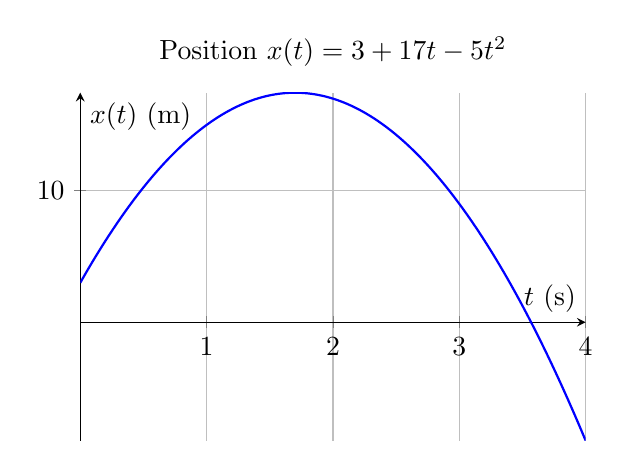
\begin{tikzpicture}
\begin{axis}[
    width=8cm,
    height=6cm,
    axis lines=middle,
    xlabel={$t$ (s)},
    ylabel={$x(t)$ (m)},
    domain=0:4,
    samples=200,
    grid=both,
    title={Position $x(t)=3+17t-5t^2$}
]
\addplot[blue, thick] {3 + 17*x - 5*x^2};
\end{axis}
\end{tikzpicture}

\vspace{1cm}

% --- Velocity v(t) ---
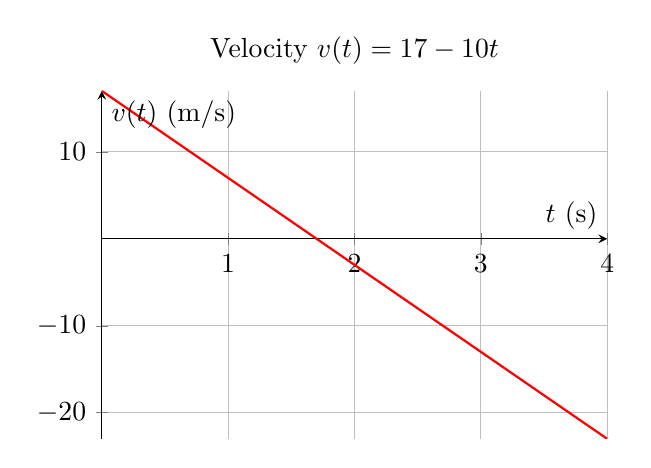
\begin{tikzpicture}
\begin{axis}[
    width=8cm,
    height=6cm,
    axis lines=middle,
    xlabel={$t$ (s)},
    ylabel={$v(t)$ (m/s)},
    domain=0:4,
    samples=200,
    grid=both,
    title={Velocity $v(t)=17-10t$}
]
\addplot[red, thick] {17 - 10*x};
\end{axis}
\end{tikzpicture}

\vspace{1cm}

% --- Acceleration a(t) ---
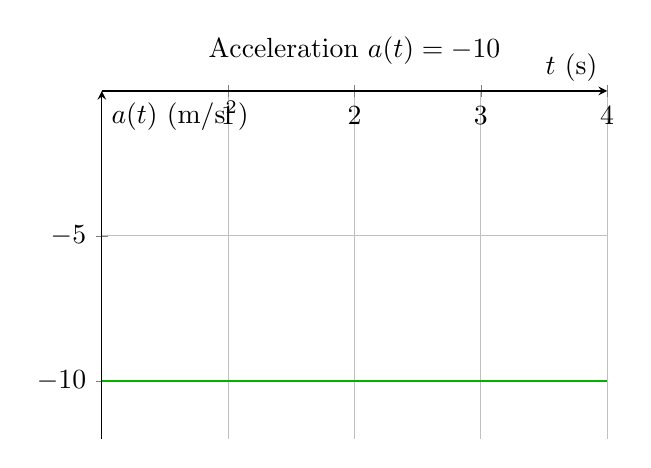
\begin{tikzpicture}
\begin{axis}[
    width=8cm,
    height=6cm,
    axis lines=middle,
    xlabel={$t$ (s)},
    ylabel={$a(t)$ (m/s$^2$)},
    domain=0:4,
    samples=2,
    grid=both,
    title={Acceleration $a(t)=-10$},
    ymin=-12, ymax=0
]
\addplot[green!70!black, thick] {-10};
\end{axis}
\end{tikzpicture}

\pagebreak 

\begin{shaded}
    (\textbf{6}) $(a)$ Determine the instantaneous acceleration of the object
    plotted in the exercise for $t = 3, t = 11$.

    $(b)$ Compute the distanace traveled by the object in the time intervals
    $[0, 5]$ and $[0, 9]$ and $[0, 15]$.

    $(c)$ Knowing that $x(t = 6) = 0$, find the position of the object at $t =
    0$. 

    $(d)$ Give an expression for the objects position for all $t$. 

    $(e)$ Plot $x(t), v(t), a(t)$.
\end{shaded}

The velocity of the object is constantly $20$m/s from time $t = 0$ to time $t =
6$. Then it linearly increases until it reaches $44$m/s at $t=9$, from whereon
it linearly decreases until it reaches $0$ms at time $t = 15$.

The linear expression $\ell_1(t) = a_1t + b_1$ which satisfies $\ell(6)=20,
\ell(9) = 44$ is such that 

\begin{equation*}
    6a_1 + b_1 = 20, \qquad 9a_1 + b_1 = 44
\end{equation*}

The associated system of equations yields that $b_1 = 20 - 6a_1$, from which
follows that $9a_1 + (20 - 6a_1) = 44$, entailing 

\begin{equation*}
    a_1 = \frac{24}{3} = 8
\end{equation*}

From this readily follows that $b_1 = 20 - 6\times 8 = -28$. 

Similarly, the linear expression $\ell_2(t) = a_2t + b_2$ which gives a line
s.t. $\ell_2(9) = 44, \ell_2(15) = 0$ must satisfy 

\begin{equation*}
    9a_2 + b_2 = 44, \qquad 15a_2 + b_2 = 0
\end{equation*}

Then $b_2 = -15a_2$ and $9a_2 -15a_2 = 44$, entailing $a_2 = -\frac{22}{3}$.
From this follows that $b_2 = 110$ via simple calculations. Thus, 


\begin{equation*}
    v(t) = \begin{cases}
        20 & 0 \leq t \leq 6 \\ 
        8t - 28 & 6 < t \leq 9 \\ 
        -\frac{22}{3}t + 110 & 9 < t \leq 15
    \end{cases}
\end{equation*}

It should be intuitive to graps that the distance travelled $d(a, b)$ in the interval
$[a, b]$ is

\begin{equation*}
    d(a, b) = \int_a^b |v(t)| ~ dt
\end{equation*}

If $v(t)$ is in meters per second, and $t$ is in seconds, the total number of
meters travelled in a time interval $[a, b]$ is the summation of the meters per
second travelled in every instant! This will involve the anti-derivative of 
$v(t)$, i.e. the movement function $x(t)$, which we might as well compute at
once. 

\begin{align*}
    x(t) 
    &= \int v(t) ~ dt \\ 
    &= \begin{cases}
        20t + C_1 & 0 \leq t \leq 6 \\ 
        8\frac{t^2}{2} - 28t + C_2 & 6 < t \leq 9 \\ 
        -\frac{22}{3} \frac{t^2}{2} + 110t + C_3 & 9 < t \leq 15
    \end{cases} \\ 
    &= \begin{cases}
        20t + C_1 & 0 \leq t \leq 6 \\ 
        4t^2 - 28t + C_2  & 6 < t \leq 9 \\ 
        -\frac{22}{6} t^2 + 110t + C_3& 9 < t \leq 15
    \end{cases}
\end{align*}

The constants $C_1, C_2, C_3$ must satisfy the restriction of continuity and of
preserving the necessary values. In particular, we need $20(0) + C_1 = 20$.
Since we know $x(6) = 0$, we need $120 + C_1 = 0$, i.e. $C_1 = -120$. We also
need 

\begin{equation*}
    4(6^2) - 28(6) + C_2 = 0
\end{equation*}

to ensure continuity, so

\begin{equation*}
    C_2 = 24
\end{equation*}

Then we can know what $x(9)$ is and deduce $C_3$, which ends up being $-597$.

\begin{equation*}
    \therefore ~ x(t) = \begin{cases}
        20t - 120 & 0 \leq t \leq 6 \\ 
        4t^2 -28t + 24 & 6 < t \leq 9 \\ 
        -\frac{22}{6}t^2 +100t - 597 & 9 < t \leq 15
    \end{cases}
\end{equation*}

In any case, we could have computed the distance travelled without $x(t)$ (I
computed $x(t)$ because it's part of the exercise):

\begin{align*}
    d(0,5) 
    &= \int_0^5 v(t) ~ dt  \\ 
    &= 20 \times t]_0^5 \\ 
    &= 20 \times (5) \\ 
    &= 100
\end{align*}

\begin{align*}
    d(0, 9) 
    &= \int_0^6 v(t) ~ dt + \int_6^9 v(t) ~ dt \\ 
    &= 20 \times t\Big]_0^6 + (4t^2 - 28t)\Big]_6^9 \\ 
    &=120 + \left[ (4 \times 81 - 28 \times 9) - (4 \times 38 - 28 \times 6)
    \right]  \\ 
    &= 120 + 96 \\ 
    &= 216
\end{align*}

etc.

\pagebreak 

\begin{shaded}
    \textbf{(7)} A car and a truck leave at the same instant, the car initially
    being a certain distance behind the truck. The latter has a constant
    acceleration of $1.2 m / s^2$, while the car accelerates at $1.8 m / s^2$. 
    The car reaches the truck when the latter has covered 45 meters. 

    $(a)$ How much time does it take for the car to reach the truck?

    $(b)$ What is the initial distance between both vehicles?

    $(c)$ What is the velocity of each in the moment the cross paths? 

    $(d)$ Plot $x(t), v(t), a(t)$.
\end{shaded}

$(a)$ Since both vehicles have constant accelerations, they have linear
velocities and therefore quadratic movement functions. They will meet 
when the parabolas corresponding to these functions intersect. 

Let $x_1(t)$ denote the movement function of the car, $x_2(t)$ that of the
truck. We then wish to find the solutions to $x_1(t) = x_2(t)$. Now, 


\begin{equation}
    v_1(t) = \int a_1(t) = \int 1.8 ~ dt = 1.8 t + C_1
\end{equation}

\begin{equation}
    v_2(t) = \int a_2(t) = \int 1.2 ~ dt = 1.2 t + C_2
\end{equation}


are the velocities of the car ($v_1$) and the truck $(v_2)$. Since at $t = 0$
the velocities of both vehicles is zero (they start from rest), it is necessary
that $C_1 = C_2 = 0$. 

We know that the car reaches the truck when the latter has covered 45 meters, so
the question is what is the time $t_0$ when the distance covered by the truck is
that one? In other words, we need to find $t_0$ such that 

\begin{align*}
&\int_0^{t_0} v_2(t) ~ dt = 45 \\ 
    \iff&\int_0^{t_0} 1.2t ~ dt = 45 \\ 
    \iff&\left[ 0.6t^2  \right]_0^{t_0} = 45 \\ 
    \iff&0.6 t_0^2  =45 \\ 
    \iff & t_0 = \sqrt{75}  = \sqrt{25 \times 3}  = 5\sqrt{3} 
\end{align*}

Thus, the vehicles meet at time $t_0 = 5\sqrt{3}  $.

$(b)$ The initial distance between both vehicles is given by $\left| x_1(0) -
x_2(0) \right| $. From the velocities $v_1, v_2$ we can determine that 

\begin{equation}
    x_1(t) = 0.9t^2 + C_1', \qquad x_2(t) = 0.6t^2 + C_2'
\end{equation}

Let us fix our coordinate system so that the starting position of the truck
corresponds to the origin. Then $C_2' = 0$. Knowing that both vehicles coincide
at time $t_0 = 5\sqrt{3} $, we also know $X_1(t_0) = x_2(t_0)$, i.e.

\begin{equation}
    0.9(25 \times 3) + C_1' = 0.6(25 \times 3) 
\end{equation}

which entails $67.5 + C_1' = 45$, from which follows  that $C_1' = -22.5$. Thus,
the original distance of both vehicles is $22.5$m.

$(c)$ This consists simply of computing $v_1(t_0), v_2(t_0)$. Trivial.

$(d)$ Meh. 

\pagebreak 

\begin{shaded}
    \textbf{(8)} A car travels parallel to a train rail. The car stops at a red
    light in the exact instant when a train passes with a constant velocity of
    12m/s. The car remains at halt for 6s and then continues with a constant
    acceleration of $2m / s^2$.

    $(a)$ Determine the time it takes for the car to reach the train, with $t =
    0$ being the instant in which the car halted. 

    $(b)$ Determine the distance traveled by the car from the red light until it
    reached the train. 

    $(c)$ Determine the car's velocity at the instant it reaches the train.
\end{shaded}

$(a)$ Let $a_1(t)$ be the acceleration of the car, defined as 

\begin{equation}
    a_1(t) = \begin{cases}
        0 & 0 \leq t < 6 \\ 
        2 & t \geq 6
    \end{cases}
\end{equation}

Let $v_2(t) = 12 m / s$ be the constant velocity of the train. Let the point of
halt be the origin of our coordinate system, so that at time $t = 0$ (when the
car halted) both the train and the car are at position zero. Observe then that
it follows that $x_2(t) = 12t$ (in meters) via integration of $v_2(t)$ and the
necessary condition of the constant of integration being zero.

Integration of equation $(6)$ gives

\begin{equation}
    v_1(t) = \begin{cases}
        C_1 & 0 \leq t < 6 \\ 
        2t + C_2 & t \geq 6
    \end{cases} 
\end{equation}

where the constants of integration must satisfy two constraints: $(a)$ $v_1(0) =
0$ and $v_1$ must be continuous. From this follows that $C_1 = 0$ and that 
$2(6) + C_2 = 0$, i.e. $C_2 = -12 $. Therefore, 

\begin{equation}
    v_1(t) = \begin{cases}
        0 & 0 \leq t < 6 \\ 
        2 t - 12 & t \geq 6
    \end{cases}
\end{equation}

Via integration of $v_1$,

\begin{equation}
    x_1(t) = \begin{cases}
        C_1' & 0 \leq t < 6 \\ 
        t^2 -12 t + C_2' & t \geq 6
    \end{cases}
\end{equation}

Again, $C_1'$ must of course be zero, and $x_1(6)$ must also be zero, meaning
that $C_2 = -36 + 12(6) = 36$. Therefore,

\begin{equation}
    x_1(t) = \begin{cases}
        0 & 0 \leq t < 6 \\ 
        t^2 -12 t + 36 & t \geq 6
    \end{cases}
\end{equation}

The car reaches the train at the time $t_0 > 6$ which satisfies $x_1(t_0) =
x_2(t_0)$, so we solve

\begin{equation*}
    t^2 - 12t + 36 = 12t \iff t^2 - 24t + 36 = 0
\end{equation*}

which has solutions

\begin{equation*}
    \frac{24}{2} \pm \frac{\sqrt{24^2 - 4 \times 36} }{2} = 12 \pm 
    \frac{\sqrt{432} }{2} \approx 12 \pm 10.392
\end{equation*}

Keeping only the positive solution, we have that $t_0 \approx 22.392$. 


$(b)$ The distance traveled by the car from the red light until it reached the
train is the distance traveled from $t = 0$ to $t = t_0$, i.e. 

\begin{equation*}
    \int_0^{t_0} v_1(t) ~ dt = |x_1(t_0) - x_1(t_0)| = x_1(t_0) \approx 268.697
\end{equation*}

where the equality above holds only because velocity is always positive (i.e.
the car moves only in one direction).

$(c)$ Simply computing $v_1(t_0)$ gives the answer.

\pagebreak 

\begin{shaded}
    \textbf{(9)} A ball is thrown vertically and upwards from the floor with
    initial velocity $v_0$. Write the equations for the movement of the ball and
    plot graphically the vectors $\vec{y}(t), \vec{v}(t), \vec{a}(t)$. Identify
    the conditions for the instant of maximum height and the instant it reaches
    the floor.
\end{shaded}

The move is strictly vertical, so $\vec{r}(t) = 0\hat{i} + y(t)\hat{j}$ and we
need only determine the unidimensional vertical movement function $y(t)$.
Now, the ball is affected only by gravitiy, i.e. it is subjected to a constant
acceleration of $\vec{a}(t) = 0\hat{i} -9.8 \frac{m}{s^2}\hat{j}$. From this we
can derive the vertical velocity: 

\begin{equation*}
    v_y(t) = -9.8 \int ~ dt = -9.8t + C
\end{equation*}

The constant of integration must satisfy the initial velocity being $v_0$, so we
must have  

\begin{equation*}
    v_y(t) = v_0 - 9.8t
\end{equation*}

From this follows that 

\begin{equation*}
    r_y(t) = \int v_0 - 9.8t ~ dt = v_0t - \frac{9.8}{2}t^2 + C'
\end{equation*}

If we assume the position on the floor (vertically) is zero, we must have 
$C' = 0$, and 

\begin{equation*}
    r_y(t) = v_0t - 4.9t^2
\end{equation*}

In summary, 

\begin{equation*}
    \vec{r}(t) = 0\hat{i} - (v_0t - 4.9t^2)\hat{j}, \qquad \vec{v}(t) = 0\hat{i}
    - 9.8t \hat{j}, \qquad \vec{a}(t) = 0 \hat{i} - 9.8 \hat{j}
\end{equation*}

Maximum hight will occur at time $t \neq 0$ when the vertical velocity of the
ball is exactly zero. So, we solve 

\begin{equation*}
    v_0 - 9.8t = 0 \iff \frac{v_0}{9.8} =t
\end{equation*}

It will reach the floor at time $t \neq 0$ when the vertical position of the
ball is zero, so we solve 

\begin{equation*}
    v_0 t - 4.9t^2 = 0 \iff t(v_0 - 4.9t) = 0
\end{equation*}

The root $t = 0$ is not a solution that interests us, so we only care about the
root that solves $v_0 - 4.9t = 0$, i.e. $t = \frac{v_0}{4.9}$.





















































\end{document}



